%definira klasu dokumenta 
\documentclass[12pt]{report} 

%prostor izmedu naredbi \documentclass i \begin{document} se zove uvod. U njemu se nalaze naredbe koje se odnose na cijeli dokument

%osnovni LaTex ne može riješiti sve probleme, pa se koriste različiti paketi koji olakšavaju izradu željenog dokumenta
\usepackage[croatian]{babel} 
\usepackage{amssymb}
\usepackage{amsmath}
\usepackage{txfonts}
\usepackage{mathdots}
\usepackage{titlesec}
\usepackage{array}
\usepackage{lastpage}
\usepackage{etoolbox}
\usepackage{tabularray}
\usepackage{color, colortbl}
\usepackage{adjustbox}
\usepackage{geometry}
\usepackage[classicReIm]{kpfonts}
\usepackage{hyperref}
\usepackage{fancyhdr}
\usepackage{graphicx}
\usepackage{caption}
\usepackage{subcaption}
\usepackage{float}
\usepackage{setspace}
\usepackage{indentfirst}
\usepackage{hyperref}
\restylefloat{table}

\patchcmd{\chapter}{\thispagestyle{plain}}{\thispagestyle{fancy}}{}{} %redefiniranje stila stranice u paketu fancyhdr

%oblik naslova poglavlja
\titleformat{\chapter}{\normalfont\huge\bfseries}{\thechapter.}{20pt}{\Huge}
\titlespacing{\chapter}{0pt}{0pt}{40pt}


\linespread{1.3} %razmak između redaka

\geometry{a4paper, left=1in, top=1in,}  %oblik stranice

\hypersetup{ colorlinks, citecolor=black, filecolor=black, linkcolor=black,	urlcolor=black }   %izgled poveznice


%prored smanjen između redaka u nabrajanjima i popisima
\newenvironment{packed_enum}{
	\begin{enumerate}
		\setlength{\itemsep}{0pt}
		\setlength{\parskip}{0pt}
		\setlength{\parsep}{0pt}
	}{\end{enumerate}}

\newenvironment{packed_item}{
	\begin{itemize}
		\setlength{\itemsep}{0pt}
		\setlength{\parskip}{0pt}
		\setlength{\parsep}{0pt}
	}{\end{itemize}}




%boja za privatni i udaljeni kljuc u tablicama
\definecolor{LightBlue}{rgb}{0.9,0.9,1}
\definecolor{LightGreen}{rgb}{0.9,1,0.9}

%Promjena teksta za dugačke tablice
\DefTblrTemplate{contfoot-text}{normal}{Nastavljeno na idućoj stranici}
\SetTblrTemplate{contfoot-text}{normal}
\DefTblrTemplate{conthead-text}{normal}{(Nastavljeno)}
\SetTblrTemplate{conthead-text}{normal}
\DefTblrTemplate{middlehead,lasthead}{normal}{Nastavljeno od prethodne stranice}
\SetTblrTemplate{middlehead,lasthead}{normal}

%podesavanje zaglavlja i podnožja

\pagestyle{fancy}
\lhead{Programsko inženjerstvo}
\rhead{Znanstvena konferencija}
\lfoot{FotoModeli}
\cfoot{stranica \thepage/\pageref{LastPage}}
\rfoot{\today}
\renewcommand{\headrulewidth}{0.2pt}
\renewcommand{\footrulewidth}{0.2pt}


\begin{document} 
	
	
	
	\begin{titlepage}
		\begin{center}
			\vspace*{\stretch{1.0}} %u kombinaciji s ostalim \vspace naredbama definira razmak između redaka teksta
			\LARGE Programsko inženjerstvo\\
			\large Ak. god. 2021./2022.\\
			
			\vspace*{\stretch{3.0}}
			
			\huge Znanstvena konferencija\\
			\Large Dokumentacija, Rev. \textit{1.0}\\
			
			\vspace*{\stretch{12.0}}
			\normalsize
			Grupa: \textit{FotoModeli}\\
			Voditelj: \textit{Marin Capan}\\
			
			
			\vspace*{\stretch{1.0}}
			Datum predaje: \textit{19. 11. 2021.}\\
	
			\vspace*{\stretch{4.0}}
			
			Nastavnik: \textit{Miljenko Krhen}\\
		
		\end{center}

	
	\end{titlepage}

	
	\tableofcontents


	\chapter{Dnevnik promjena dokumentacije}
		
		\textbf{\textit{Kontinuirano osvježavanje}}\\
				
		
		\begin{longtblr}[
				label=none
			]{
				width = \textwidth, 
				colspec={|X[2]|X[13]|X[3]|X[3]|}, 
				rowhead = 1
			}
			\hline
			\textbf{Rev.}	& \textbf{Opis promjene/dodatka} & \textbf{Autori} & \textbf{Datum}\\[3pt] \hline
			0.1 & Popunjena naslovnica i napravljen predložak.	& P.D.Grujić Ostojić, A.Sambolek & 18.10.2021. 		\\[3pt] \hline
			0.2 & Dodani funkcionalni zahtjevi korisnika.			& R.Pintar, A.Sambolek & 27.10.2021.		\\[3pt]\hline
			0.3 & Dodani obrasci uporabe i opis projektnog zadatka		& R.Pintar, J.Gavran & 30.10.2021.		\\[3pt]\hline
			0.4 & Ažuriran dnevnik sastajanja		& P.D.Grujić Ostojić & 31.10.2021.		\\[3pt]\hline
			&  &  & \\[3pt] \hline	
		\end{longtblr}
	
	
		\textit{Moraju postojati glavne revizije dokumenata 1.0 i 2.0 na kraju prvog i drugog ciklusa. Između tih revizija mogu postojati manje revizije već prema tome kako se dokument bude nadopunjavao. Očekuje se da nakon svake značajnije promjene (dodatka, izmjene, uklanjanja dijelova teksta i popratnih grafičkih sadržaja) dokumenta se to zabilježi kao revizija. Npr., revizije unutar prvog ciklusa će imati oznake 0.1, 0.2, …, 0.9, 0.10, 0.11.. sve do konačne revizije prvog ciklusa 1.0. U drugom ciklusu se nastavlja s revizijama 1.1, 1.2, itd.}
	\chapter{Opis projektnog zadatka}
		
		\textbf{\textit{dio 1. revizije}}\\

		Znanstvena udruga “Pametna ekipa” organizira konferenciju na kojoj će sudionici prezentirati svoje radove. Cilj ovog projekta je razviti učinkovit informacijski sustav koji će podržati istovremeni rad više korisnika i ovisno o njihovoj ulozi omogućiti im različite funkcionalnosti. Sudionicima treba omogućiti prijavu na konferenciju i predaju rada s kojim žele sudjelovati, recenzentima da recenziraju zaprimljene radove sudionika, administratoru definiranje upitnika za prijavu i upravljanje sadržajem na samoj web aplikaciji, a predsjedavajućem konferencije da odobrava recenzente te općenito nadgleda podatke sudionika i njihove radove. Dodatno, administrator na web aplikaciji može vidjeti informacije o trenutnoj epidemiološkoj situaciji u državama iz kojih ima prijavljenih sudionika te po potrebi učiniti radove javno dostupnima.
		\newline
		\newline
		Prilikom pokretanja sustava, neregistriranom odnosno neprijavljenom korisniku prikazuje se naslovnica na kojoj se nalazi statičan sadržaj te gumb koji vodi do stranice za registraciju/prijavu. Na vrhu svake stranice  je postavljena traka koja korisniku omogućuje brzo preusmjeravanje na određene stranice: naslovnica, pristup radovima, stranica s kontaktima, te stranica za prijavu u sustav ili profil korisnika ako je korisnik već prijavljen. U slučaju pogoršanja epidemiološke situacije svi će prijavljeni korisnici imati pristup svim odobrenim radovima, a do tada pristup svim radovima imaju samo administrator i predsjedavajući konferencije. Statični sadržaj na početnoj stranici odnosi se na informacije o konferenciji te članke i radove vezane uz konferenciju. Članci nisu cjelovito prikazani, stoga se ispod svakog nalazi gumb "Saznaj više" koji korisnika preusmjerava na stranicu koja sadrži cjelovit članak. Na naslovnici se nalazi i dinamičan okvir koji prikazuje sliku sa poveznicom na istaknuti članak. Okvir može mijenjati sliku i poveznicu korisnikovim gumbom na strelicu. Pri ulasku na samu naslovnicu, ukoliko korisnik nije prijavljen, u dinamičnom se okviru pojavljuje veliki gumb "\textit{Registracija}" koji korisnika preusmjerava na registraciju u sustav. 
		\newline
		\newline
		Na stranici za prijavu nalazi se okvir u koji već registrirani korisnici unose korisničko ime i lozinku, a ispod se nalazi gumb koji preusmjerava neregistrirane korisnike na formu za registraciju. Također se ispod okvira nalazi i gumb "\textit{Zaboravljena lozinka}" koji korisniku omogućava slanje nove lozinke na e-mail adresu koju unese. Na stranici za registraciju, odnosno prijavu na konferenciju, postoje dvije opcije: \textit{Registriraj se kao sudionik} i \textit{Registriraj se kao recenzent}. Administrator i predsjedavajući konferencije ne vrše registraciju, već postoji jedan unaprijed definiran administrator koji, ako želi, u sustav dodaje druge administratore čije se funkcionalnosti ne razlikuju od "prvog" administratora. Administrator također određuje predsjedavajućeg konferencije kojemu se na e-mail šalju podatci za prijavu u sustav.
		\newline
		\newline
		Pri registraciji sudionika konferencije potrebni su sljedeći podaci:

		\begin{packed_item}

			\item ime
			\item prezime
			\item e-mail adresa
			\item matična ustanova (institucija ili poduzeće) i adresa iste - ulica i kućni broj, grad, država
			\item sekcija u kojoj žele sudjelovati/recenzirati radove koju korisnik odabire iz ponuđene liste
			\item potrebno je odabrati prijavljuje li se osoba kao sudionik ili recenzent
			\item naslov rada (samo za sudionike)
			\item imena autora rada (samo za sudionike)
			\item e-mail adresa autora kojeg korisnik označi kao osobu za kontakt
		
		\end{packed_item}
	
		U slučaju da neki od podataka nije upisan, sustav javlja kako nisu svi podaci uneseni i traži od korisnika da ih unese ukoliko se želi registrirati. Također se vrši provjera postoji li već u bazi podataka rad istog naslova i autora. Nakon izvršene registracije, ovisno o tome koju ulogu je korisnik odabrao (sudionik ili recenzent) dobit će određena prava koja su objašnjena u nastavku. Korisnik na unesenu e-mail adresu prima poruku o uspješnoj prijavi, te se u poruci nalazi lozinka i korisničko ime koji su potrebni za prijavu u sustav te link na koji mora kliknuti kako bi potvrdio uspješnu registraciju. Sudionici konferencije bi trebali učitati svoj rad u sustav do datuma roka za prijavu na konferenciju koji je javno dostupan.
		\newline
		\newline
		Svaki registrirani korisnik, bez obzira na razinu ovlasti, može pregledavati vlastite korisničke podatke i mijenjati ih po potrebi, osim e-mail adrese i lozinke. 
		\newline
		\newline
		Postoje četiri vrste registriranih korisnika:
		
		\begin{packed_item}
			
			\item administrator
			\item predsjedavajući konferencije
			\item recenzent
			\item sudionik konferencije
			
		\end{packed_item}
	
		\underline{\textit{Administrator}} sustava ima najveću razinu ovlasti. Prilikom samog pokretanja sustava, postoji jedan unaprijed definiran administrator koji, ako želi, u sustav dodaje druge administratore te određuje predsjedavajućeg konferencije. Administrator može mijenjati statički sadržaj na naslovnici, unosi podatke o konferenciji, primjerice definira rok prijave na konferenciju i sekcije u kojima sudionici mogu sudjelovati te definira upitnik za prijavu na konferenciju. U slučaju pogoršane epidemiološke situacije, administrator može dio ili sve radove učiniti javno dostupnima te o tome obavijestiti pojedine (ili sve) sudionike konferencije.
		
		
		\underline{\textit{Predsjedavajući konferencije}} ima glavnu ulogu odobravanja recenzenata. \textit{(na koji način?)} Osim svojih podataka, on također ima uvid u osobne podatke svih sudionika, te ih po potrebi može mijenjati. Također ima mogućnost preuzimanja radova svih sudionika na vlastito računalo. Isto tako, ukoliko se pokaže potreba, može poslati pojedinačnim sudionicima e-mail ili ga pak poslati svim sudionicima konferencije. 
		
		
		\underline{\textit{Recenzent}} je osoba koja recenzira odnosno kontrolira radove sudionika. Svaki rad pregledava samo jedan recenzent, a svaki recenzent može pregledati više radova iz sekcije koju odabere pri prijavi i samo iz te sekcije. Pregledavanjem i recenziranjem radova recenzent odobrava sudjelovanje sudionika na konferenciji. Radove može pregledavati \textit{online} ili ih može preuzeti na računalo i pregledavati. 
		
		Nakon pregleda pojedinog rada, recenzent ima sljedeće mogućnosti:
		
		\begin{enumerate}
			
			\item prihvaćanje rada bez potrebnih izmjena i/ili dopuna rada
			\item prihvaćanje rada, ali sudionik prije finalne predaje mora napraviti manje dorade koje recenzent ne mora provjeriti
			\item prihvaćanje rada, ali uz potrebne značajne izmjene rada o kojima, nakon izvršenja, sudionik mora obavijestiti recenzenta radi njihove provjere
			\item potpuno odbijanje rada uz obrazloženje
			
		\end{enumerate}
	
		\underline{\textit{Sudionik}} ima najmanju razinu ovlasti - on jedino ima mogućnost pregledavanja i izmjene osobnih podataka te učitavanje radova u sustav. Za njega je glavna svrha sustava upravo prijava na konferenciju i učitavanje rada s kojim želi sudjelovati. Nakon prijave i učitavanja rada u sustav, korisnik ima mogućnost prijaviti još svojih radova.
		
		Na internetu se može pronaći mnoštvo odličnih, ali i manje dobrih, primjera sustava za prijavu na različite konferencije. Kod ovakvih sustava važno je da su intuitivni kako bi korisnik lako došao do potrebnih informacija vezanih uz konferenciju i sudjelovanje na njoj. Nije zanemariva ni estetska komponenta web-sučelja jer je jedna od osnovnih svrha ove programske potpore privući potencijalne sudionike, a možda i sponzore. U nastavku navodimo par rješenja koja su nas se dojmila te nam mogu poslužiti kao vodilja u osmišljavanju vlastita sustava.
	
		\eject
		
	
	\chapter{Specifikacija programske potpore}
		
	\section{Funkcionalni zahtjevi}
			
			\textbf{\textit{dio 1. revizije}}\\
			
			
			\noindent \textbf{Dionici:}
			
			\begin{packed_enum}
				
				\item Sudionici konferencije
				\item Recenzenti
				\item Predsjedavajući konferencije				
				\item Administrator sustava
				
			\end{packed_enum}
			
			\noindent \textbf{Aktori i njihovi funkcionalni zahtjevi:}
			
			
			\begin{packed_enum}
				\item  \underbar{Neregistriran/neprijavljen korisnik (inicijator) može:}
				
				\begin{packed_enum}
					
					\item pristupiti naslovnici konferencije i sadržaju na njoj, kao i stranici s informacijama o samoj konferenciji
					\item prijaviti se u sustav, a ako to još nije napravio može se registrirati - stvoriti novi korisnički račun za koji su mu potrebni osobni podaci - ime i prezime, naziv matične ustanove (kao i ulica i kućni broj, grad i država institucije), e-mail adresa te ovisno o odabiru uloge autore rada (sudionici)
					\item prilikom prijave zatražiti novu lozinku
					
				\end{packed_enum}
			
				\item  \underbar{Sudionik (inicijator) može:}
				
				\begin{packed_enum}
					
					\item pregledavati i mijenjati osobne podatke (osim e-maila i lozinke)
					\item učitati rad u .pdf formatu (do kraja roka za predaju)
					\item po potrebi priložiti izmijenjenu verziju rada i pri tome obavijestiti recenzenta u učinjenome
					
					
				\end{packed_enum}
				
				\item  \underbar{Recenzent (inicijator) može:}
				
				\begin{packed_enum}
					
					\item pregledavati i mijenjati osobne podatke (osim e-maila i lozinke)
					\item dohvaćati pristigle radove
					\item preuzeti radove na lokalno računalo
					\item prihvatiti rad bez izmjena
					\item prihvatiti rad uz manje izmjene, bez naknadnih provjera
					\item odobriti rad uz veće izmjene, pri čemu mora obavijestiti autora te ponovno pregledati izmijenjeni rad
					\item u potpunosti odbiti rad, pri čemu je potrebno navesti razloge i objasniti ocjenu
					
					
				\end{packed_enum}
				
				\item  \underbar{Predsjedavajući konferencije (inicijator) može:}
				
				\begin{packed_enum}
				
					\item vidjeti sve podatke o sudionicima, mijenjati ih i dodavati sadržaj
					\item preuzeti sve pristigle radove na lokalno računalo
					\item dati odobrenje za obavljanje recenzije radova recenzentima
					\item svima ili samo odabranim korisnicima slati obavijesti na e-mail
				
				\end{packed_enum}
				
				\item  \underbar{Administrator (inicijator) može:}
				
				\begin{packed_enum}
				
					\item upisati podatke o konferenciji
					\item odrediti predsjedavajuče članove konferencije
				\end{packed_enum}

				\item \underbar{Baza podataka (sudionik):}

				\begin{packed_enum}

					\item pohranjuje podatke o korisnicima te njihovim ulogama i ovlastima u sustavu
					\item pohranjuje podatke o radovima, njihovim autorima i recenzijama tih radova

				\end{packed_enum}
					
			\end{packed_enum}
			
			\eject 
			
			
				
			\subsection{Obrasci uporabe}
				
				\textbf{\textit{dio 1. revizije}}
				
				\subsubsection{Opis obrazaca uporabe}
					
					\noindent \underbar{\textbf{UC1 - Pregled naslovnice}}
					\begin{packed_item}
	
						\item \textbf{Glavni sudionik: } Neprijavljeni korisnik, sudionik, recenzent
						\item  \textbf{Cilj:} Pregledavanje statičnog sadržaja naslovnice
						\item  \textbf{Sudionici:} Baza podataka
						\item  \textbf{Preduvjet:} -
						\item  \textbf{Opis osnovnog tijeka:}
						
						\item[] \begin{packed_enum}
	
							\item Na naslovnici se prikazuje statičan sadržaj, odnosno činjenice i informacije o konferenciji i sl.
							\item Neprijavljeni korisnici te prijavljeni sudionici i recenzenti mogu pregledavati spomenute sadržaje
						\end{packed_enum}
						
%ovaj dio je ostavljen iz razloga da ga se moze prekopirat za ostale obrasce uporabe
						\item  \textbf{Opis mogućih odstupanja:}
						
						\item[] \begin{packed_item}
	
							\item[2.a] $<$opis mogućeg scenarija odstupanja u koraku 2$>$
							\item[] \begin{packed_enum}
								
								\item $<$opis rješenja mogućeg scenarija korak 1$>$
								\item $<$opis rješenja mogućeg scenarija korak 2$>$
								
							\end{packed_enum}
							\item[2.b] $<$opis mogućeg scenarija odstupanja u koraku 2$>$
							\item[3.a] $<$opis mogućeg scenarija odstupanja  u koraku 3$>$
							
						\end{packed_item}
					\end{packed_item}

					\noindent \underbar{\textbf{UC2 - Registracija}}
					\begin{packed_item}
	
						\item \textbf{Glavni sudionik: } Neprijavljeni korisnik
						\item  \textbf{Cilj:} Stvaranje novog korisničkog računa za pristup aplikaciji
						\item  \textbf{Sudionici:} Baza podataka
						\item  \textbf{Preduvjet:} -
						\item  \textbf{Opis osnovnog tijeka:}
						
						\item[] \begin{packed_enum}
	
							\item Korisnik odabire opciju za registraciju
							\item Korisnik unosi osobne podatke potrebne za registraciju
							\item Nakon upisanih osobnih podataka, korisnik odabire kreira li račun kao sudionik ili recenzent, te ukoliko odabere opciju sudionik pojavljuje se još jedan dio obrasca gdje je potrebno unijeti naziv rada koji želi predati i autore istog
							\item Nakon registracije i nakon što administrator odobri prijavu, korisnik prima obavijest (putem e-maila) o uspješnoj registraciji u kojoj se nalazi lozinka s kojom se prijavljuje u sustav
						\end{packed_enum}

						\item  \textbf{Opis mogućih odstupanja:}
						
						\item[] \begin{packed_item}
	
							\item[2.a]  Odabir već zauzetog korisničkog imena i/ili e-maila, unos jednog ili više korisničkih podataka u nedozvoljenom formatu
							\item[] \begin{packed_enum}
								
								\item Sustav korisniku daje obavijest o tome gdje je nastala greška pri registraciji
								\item Korisnik sukladno mijenja unesene podatke sve dok nisu svi potrebni podaci ispravno upisani, odnosno u odgovarajućem formatu
								
							\end{packed_enum}
							
						\end{packed_item}
			
					\end{packed_item}
				
					
				\subsubsection{Dijagrami obrazaca uporabe}
					
					\textit{Prikazati odnos aktora i obrazaca uporabe odgovarajućim UML dijagramom. Nije nužno nacrtati sve na jednom dijagramu. Modelirati po razinama apstrakcije i skupovima srodnih funkcionalnosti.}
				\eject		
				
			\subsection{Sekvencijski dijagrami}
				
				\textbf{\textit{dio 1. revizije}}\\
				
				\textit{Nacrtati sekvencijske dijagrame koji modeliraju najvažnije dijelove sustava (max. 4 dijagrama). Ukoliko postoji nedoumica oko odabira, razjasniti s asistentom. Uz svaki dijagram napisati detaljni opis dijagrama.}
				\eject
	
		\section{Ostali zahtjevi}
		
			\textbf{\textit{dio 1. revizije}}\\
		 
			 \textit{Nefunkcionalni zahtjevi i zahtjevi domene primjene dopunjuju funkcionalne zahtjeve. Oni opisuju \textbf{kako se sustav treba ponašati} i koja \textbf{ograničenja} treba poštivati (performanse, korisničko iskustvo, pouzdanost, standardi kvalitete, sigurnost...). Primjeri takvih zahtjeva u Vašem projektu mogu biti: podržani jezici korisničkog sučelja, vrijeme odziva, najveći mogući podržani broj korisnika, podržane web/mobilne platforme, razina zaštite (protokoli komunikacije, kriptiranje...)... Svaki takav zahtjev potrebno je navesti u jednoj ili dvije rečenice.}
			 
			 
			 
	
	\chapter{Arhitektura i dizajn sustava}
		
	
		Arhitektura sustava je izvedena u obliku web aplikacije kojoj korisnik pristupa koristeći web preglednik. Web preglednik omogućuje korisniku pregled web-stranica i multimedijskog sadržaja na njima. Postoje razni web preglednici za različite operacijske sustave te ovaj pristup omogućava lak i širok pristup aplikaciji bez potrebe za dodatnim preuzimanjem programske podrške od strane korisnika.
	\par Za razvoj aplikacije koristimo programski jezik Python, HTML, JavaScript i CSS. Koristimo razvojno okruženje Django koje smo odabrali zbog njegove jednostavnosti, modularnosti te upoznatosti tima s razvojem u toj okolini.
Korisnik vrši interakcije sa aplikacijom preko Django predložaka. Predlošci (eng. \textit{templates}) sadrže strukturu potrebnu za dinamičko generiranje HTML stranice i prikaz iste korisniku.



	\begin{figure}[H]
						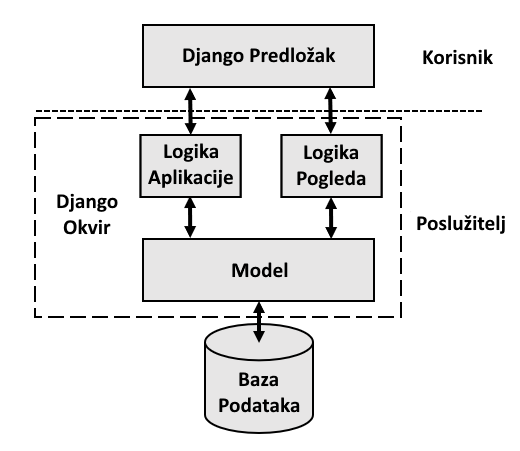
\includegraphics[scale=0.9]{dijagrami/django.png} 
						\centering
						\caption{Dijagram načina rada Djanga}
						\label{fig:dijagramRadaDjanga}
					\end{figure}

		Django predlošci su jedan od sastavnih dijelova radnog okvira Django. Django funkcionira na MVT principu rada, koji je strukturno vrlo sličan modelu MVC.\newline MVT model se sastoji od:
\begin{itemize}
		\item 	\textbf{Model} - objekti u Pythonu koji definiraju strukturu podataka aplikacije i omogućavaju dodavanje, brisanje, mijenjanje i dohvaćanje podataka iz baze podataka.
		\item 	\textbf{View (pogled)} - funkcije koje sluze za obradu HTTP zahtjeva i generiranje HTTP odziva. Pogledi pristupaju podatcima potrebnima za odrađivanje zahtjeva uz pomoć modela, a za formatiranje i prikaz  dohvaćenih podataka koriste predloške.
		\item 	\textbf{Template (predložak)} - definira strukturu prikaza podataka neke datoteke (npr. HTML). Pogledi mogu dinamički generirati HTML stranice uz pomoć predložaka i popuniti ih s podacima dohvaćenih putem modela. 
				
	\end{itemize}

		\begin{figure}[H]
						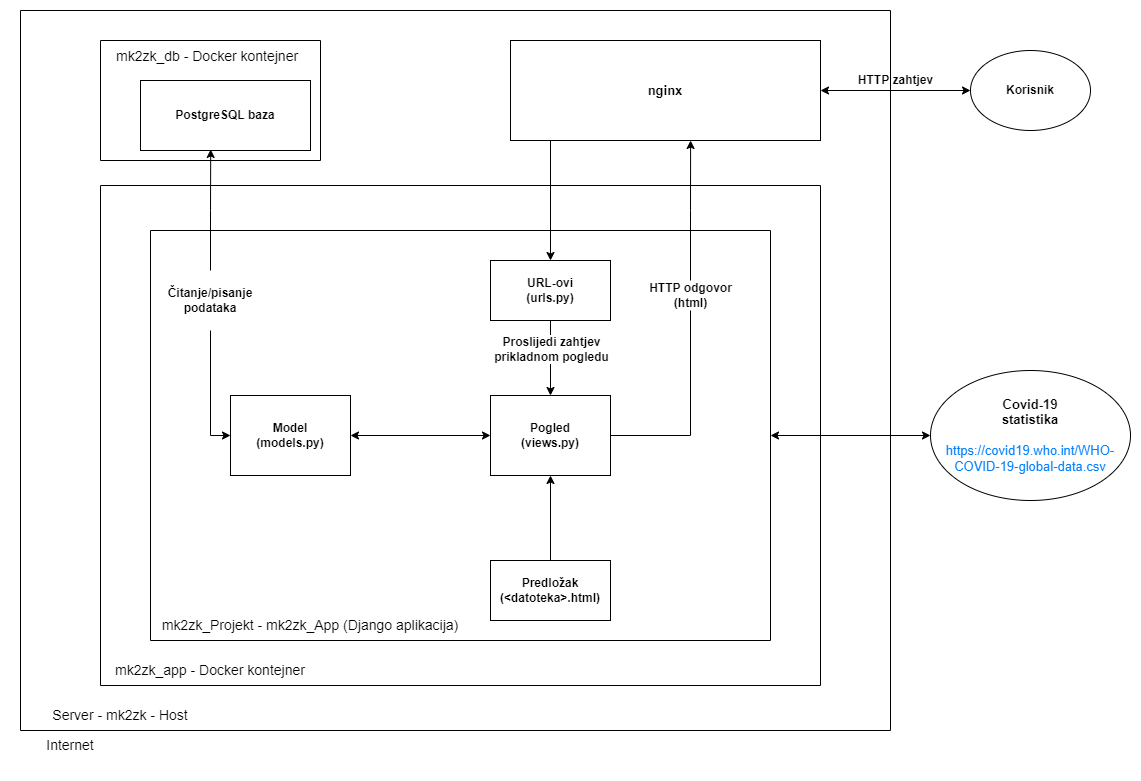
\includegraphics[scale=0.9]{dijagrami/django_mvt.png} 
						\centering
						\caption{Dijagram principa rada MVT}
						\label{fig:dijagramRadaMVT}
					\end{figure}

		

				
		\section{Baza podataka}
			
			\textbf{\textit{dio 1. revizije}}\\
			
			Baze podataka neizostavan su dio razvoja programske potpore jer danas gotova svaka domena primjene djeluje mnoštvom podataka koje treba pohraniti na organiziran način kako bi se efikasno dohvaćali, mijenjali i nadopunjavali. Za upravljanje bazom podataka mogu se koristiti različiti sustavi koji obavljaju optimiranje upita i omogućuju rukovanje podacima. Mi smo odlučili koristiti PostgreSQL koji nam je bio preporučen na kolegiju Baze podataka. \newline Iako stvarni svijet ne možemo prikazati sa svim detaljima, relacijski nam model baze podataka omogućuje vjeran prikaz stvarnosti pomoću relacija u koje pohranjujemo vrijednosti odabranih atributa koji su vezani uz entitete bitne za domenu primjene. Formalno gledano relacija, odnosno instanca relacije, definirana na relacijskoj shemi je skup n-torki, a neformalno možemo reći da je to imenovana dvodimenzionalna tablica. Atributi su imenovani stupci te tablice. ER (\textit{Entity-Relationship}) model podataka zadržava dobra svojstva relacijskog modela, a uz to omogućuje eksplicitni prikaz semantičkih informacija vezanih uz veze (odnose) između entiteta. ER dijagram prikazuje kako su entiteti našeg sustava povezani. Pri preslikavanju ER modela u relacijski model, entiteti i veze postaju entiteti (relacije) te se sheme s jednakim ključevima zamjene njihovom unijom.
		Baza podataka ove aplikacije sastoji se od sljedećih entiteta:
		\begin{packed_item}
			\item Korisnik
			\item Rad
			\item Autor
			\item AutorRad
			\item Sekcija
			\item Uloga
			\item Konferencija
			\item DodatnoPoljeObrasca
			\item TipPoljeObrasca
			\item DodatniPodatak 
			\item Recenzija
			\item Ocjena
			\item Ustanova
		\end{packed_item}
		
			\subsection{Opis tablica}
			

				\textbf{Korisnik}
				Ovaj entitet sadržava sve važne informacije (atribute) o svim korisnicima aplikacije: korisničko ime, e-mail, lozinku, ime, prezime te ulogu korisnika u sustavu. Atributi token i potvrdioPrijava služe kako bi se za sudionike i recenzente provjerilo jesu li potvrdili prijavu (nakon čega se mogu prijaviti u sustav). Atribut sudionikID je svojstven korisnicima koji su sudionici, a atribut odobren i sifSekcija je svojstven recenzentima. Ovaj entitet je u vezi \begin{packed_item} 
					\item Many-to-One s entitetom Ustanova preko atributa ID
					\item Many-to-One s entitetom Sekcija preko atributa ID
					\item Many-to-One s entitetom Uloga preko atributa ID
					\item One-to-Many s entitetom Recenzija preko atributa ID (Recenzija.recezentID)
					\item Many-to-Many s entitetom DodatnoPoljeObrasca preko atributa ID (DodatniPodatak.korisnikID; ta je veza na ER dijagramu imenovana kao DodatniPodatak pa se može reći da je entitet Korisnik u vezi One-to-Many s entitetom DodatniPodatak preko atributa ID)
					\item One-to-Many s entitetom Rad preko atributa ID (Rad.prijavioID)
				\end{packed_item}
				\begin{longtblr}[
					label=none,
					entry=none
					]{
						width = \textwidth,
						colspec={|X[7,l]|X[6, l]|X[20, l]|}, 
						rowhead = 1,
					} %definicija širine tablice, širine stupaca, poravnanje i broja redaka naslova tablice
					\hline \multicolumn{3}{|c|}{\textbf{Korisnik}}	 \\ \hline[3pt]
					\SetCell{LightGreen}ID & INT	&  jedinstveni brojčani identifikator	\\ \hline
					korisnickoIme	& VARCHAR & korisnički identifikator  kojeg korisnik koristi pri prijavi u sustav	\\ \hline 
					email & VARCHAR & adresa e-pošte korisnika  \\ \hline 
					lozinka & VARCHAR & hash lozinke  \\ \hline 
					ime & VARCHAR	&  	ime korisnika	\\ \hline 
					prezime & VARCHAR & prezime korisnika  \\ \hline 
					sudionikID & INT & jedinstvena oznaka sudionika (ID\_XXXX, 
					pri čemu je XXXX redni broj prijave)\\ \hline 
					odobren & BOOLEAN & oznaka je li predsjedavajući konferencije odobrio recenzenta\\ \hline 
					token & VARCHAR & link koji se šalje sudionicima i recenzentima na e-mail kako bi klikom na njega potvrdili svoju prijavu  \\ \hline
					potvrdioPrijava & BOOLEAN & oznaka je li korisnik (sudionik/recenzent) potvrdio svoju prijavu\\ \hline  
					\SetCell{LightBlue} sifUstanova	& INT & jedinstvna brojčana oznaka matične ustanove korisnika (Ustanova.ID)  	\\ \hline 
					\SetCell{LightBlue} sifSekcija	& INT & jedinstvena brojčana oznake sekcije (Sekcija.ID) u kojoj je
					recenzent odabrao recenzirati radove	\\ \hline 
					\SetCell{LightBlue} ulogaKorisnik	& INT & oznaka korisnikove uloge u sustavu (Uloga.ID) \\ \hline 
				\end{longtblr}
				\textbf{Ustanova} Ovaj entitet predstavlja ustanove (poduzeća ili institucije) kojima pripadaju prijavljeni sudionici i recenzenti. Atributi ovog entiteta su: ID, naziv, grad, država i adresa ustanove. Entitet je u vezi
				\begin{packed_item}
					\item One-to-Many s entitetom Korisnik preko atributa sifUstanova (jedinstveni brojčani identifikator ustanove; Korisnik.sifUstanova).	
				\end{packed_item} 
				\begin{longtblr}[
					label=none,
					entry=none
					]{
						width = \textwidth,
						colspec={|X[6,l]|X[6, l]|X[20, l]|}, 
						rowhead = 1,
					} %definicija širine tablice, širine stupaca, poravnanje i broja redaka naslova tablice
					\hline \multicolumn{3}{|c|}{\textbf{Ustanova}}	 \\ \hline[3pt]
					\SetCell{LightGreen}ID & INT	&  jedinstveni brojčani identifikator	\\ \hline
					naziv	& VARCHAR &   naziv ustanove	\\ \hline 
					grad & VARCHAR & grad u kojem je ustanova  \\ \hline 
					drzava & VARCHAR	&  država u kojoj je ustanova		\\ \hline 
					adresa & VARCHAR	&  adresa ustanove		\\ \hline 
					
				\end{longtblr}
				\textbf{Uloga}
				Ovaj entitet predstavlja ulogu koju korisnik sustava može imati. U ovom sustavu razlikujemo 4 uloge: sudionik, administrator, predsjedavajući konferencije i recenzent. Svaki korisnik ima samo jednu ulogu. Atributi ovog entiteta su: ID i naziv uloge. Entitet je u vezi:
				\begin{packed_item}
					\item One-to-Many s entitetom Korisnik preko atributa ID (Korisnik.ulogaKorisnik)
				\end{packed_item}
				\begin{longtblr}[
					label=none,
					entry=none
					]{
						width = \textwidth,
						colspec={|X[6,l]|X[6, l]|X[20, l]|}, 
						rowhead = 1,
					} %definicija širine tablice, širine stupaca, poravnanje i broja redaka naslova tablice
					\hline \multicolumn{3}{|c|}{\textbf{Uloga}}	 \\ \hline[3pt]
					\SetCell{LightGreen}ID & INT	& jedinstveni brojčani identifikator	\\ \hline
					naziv	& VARCHAR &   naziv uloge	\\ \hline 
					
				\end{longtblr}
				
				\textbf{Ocjena}
				Ovaj entitet predstavlja ocjenu kojom recenzenti mogu ocijeniti neki rad. Početno, u sustavu razlikujemo 4 ocjene (4 jedinstvena brojčana identifikatora) čije se značenje razlikuje (prihvaćanje rada, prihvaćanje rada uz manju doradu, prihvaćanje rada uz veću doradu, neprihvaćanje rada). Ovaj entitet je u vezi 	\begin{packed_item} 
					\item One-to-Many s entitetom Recenzija preko atributa ID (Recenzija.ocjena)
				\end{packed_item}
				\begin{longtblr}[
					label=none,
					entry=none
					]{
						width = \textwidth,
						colspec={|X[6,l]|X[6, l]|X[20, l]|}, 
						rowhead = 1,
					} %definicija širine tablice, širine stupaca, poravnanje i broja redaka naslova tablice
					\hline \multicolumn{3}{|c|}{\textbf{Ocjena}}	 \\ \hline[3pt]
					\SetCell{LightGreen}ID & INT	& jedinstveni brojčani identifikator	\\ \hline
					znacenje	& VARCHAR &   značenje odabrane ocjene	\\ \hline 
					
				\end{longtblr}
				\textbf{Sekcija}
				Ovaj entitet predstavlja sekcije na konferenciji. Na znanstvenoj konferenciji koju modeliramo može biti više sekcija, recenzent recenzira radove unutar jedne sekcije, a svaki rad pripada točno jednoj sekciji. Identifikator entiteta je atribut ID. Entitet sadrži informaciju o nazivu sekcije i u vezi je
				\begin{packed_item}
					\item Many-to-One s entitetom Konferencija preko atributa ID
					\item One-to-Many s entitetom Korisnik preko atributa ID (Korisnik.sifSekcija)
					\item One-to-Many s entitetom Rad preko atributa ID (Rad.sifSekcija)
				\end{packed_item} 
				\begin{longtblr}[
					label=none,
					entry=none
					]{
						width = \textwidth,
						colspec={|X[7,l]|X[6, l]|X[20, l]|}, 
						rowhead = 1,
					} %definicija širine tablice, širine stupaca, poravnanje i broja redaka naslova tablice
					\hline \multicolumn{3}{|c|}{\textbf{Sekcija}}	 \\ \hline[3pt]
					\SetCell{LightGreen}ID & INT	&  	jedinstveni brojčani identifikator	\\ \hline
					naziv	& VARCHAR &   naziv konferencije	\\ \hline 
					\SetCell{LightBlue} sifKonferencija	& INT &   jedinstveni brojčani identifikator konferencije (Konferencija.ID)	\\ \hline
					
				\end{longtblr}
				\textbf{Konferencija}
				Ovaj entitet sadrži važne informacije o znanstvenoj konferenciji koju modeliramo. Atributi su: identifikator konferencije (ID), naziv konferencije, opis, datum održavanja, rok za prijave, rok za administracijske promjene, rok za recenzente. Entitet je u vezi
				\begin{packed_item}
					\item One-to-Many s entitetom Sekcija preko atributa ID (Sekcija.sifKonferencija)
					
				\end{packed_item}
				\begin{longtblr}[
					label=none,
					entry=none
					]{
						width = \textwidth,
						colspec={|X[8,l]|X[6, l]|X[20, l]|}, 
						rowhead = 1,
					} %definicija širine tablice, širine stupaca, poravnanje i broja redaka naslova tablice
					\hline \multicolumn{3}{|c|}{\textbf{Konferencija}}	 \\ \hline[3pt]
					\SetCell{LightGreen}ID & INT	& jedinstveni brojčani identifikator	\\ \hline
					naziv	& VARHCAR & naziv konferencije  	\\ \hline 
					opis & VARCHAR &  opis konferencije \\ \hline
					datum & DATE &  datum održavanja konferencije \\ \hline 
					rokPrijava & TIMESTAMP &  rok za prijavu na konferenciju i učitanje rada u sustav \\ \hline 
					rokAdmin & TIMESTAMP &  rok do kojeg administrator može mijenjati obrazac za prijavu \\ \hline 
					rokRecenzent & TIMESTAMP &  rok do kojeg recenzenti mogu (trebaju) obaviti recenziju radova \\ \hline
					pocetakRecenzent & TIMESTAMP & vremenski trenutak od kojeg recenzenti mogu recenzirati radove  \\ \hline
					pocetakPrijava & TIMESTAMP & vremenski trenutak od kojeg se sudionici i recenzenti mogu početi prijavljivati na konferenciju  \\ \hline
					
					
				\end{longtblr}
				
				\textbf{DodatnoPoljeObrasca} Ovaj entitet sadrži informacije o dodatnim poljima obrasca koja se nude administratoru pri definiranju obrasca za prijavu na konferenciju. Atributi su: ID (jedinstveni identifikator), naziv polja, tip polja, oznake obavezno i prisutno. Entitet je u vezi
				\begin{packed_item}
					\item Many-to-One s entitetom TipPoljeObrasca preko atributa ID
					\item Many-to-Many s entitetom Korisnik preko atributa ID \newline (DodatniPodatak.poljeObrascaID; ta je veza na ER dijagramu imenovana kao DodatniPodatak pa se može reći da je entitet DodatnoPoljeObraca u vezi One-to-Many s entitetom DodatniPodatak preko atributa ID)
				\end{packed_item} 
				\begin{longtblr}[
					label=none,
					entry=none
					]{
						width = \textwidth,
						colspec={|X[6,l]|X[6, l]|X[20, l]|}, 
						rowhead = 1,
					} %definicija širine tablice, širine stupaca, poravnanje i broja redaka naslova tablice
					\hline \multicolumn{3}{|c|}{\textbf{DodatnoPoljeObrasca}}	 \\ \hline[3pt]
					\SetCell{LightGreen}ID & INT	&  jedinstveni brojčani identifikator 	\\ \hline
					ime	& VARCHAR & ime dodatnog polja obrasca  	\\ \hline 
					\SetCell{LightBlue}tipPolje	& INT & tip dodatnog polja obrasca  	\\ \hline 
					obavezno	& BOOLEAN & oznaka je li polje obavezno polje obrasca	\\ \hline
					prisutno	& BOOLEAN & oznaka treba li polje biti prisutno u obrascu	\\ \hline
					
				\end{longtblr}
				\textbf{TipPoljeObrasca}
				Ovaj entitet sadrži informacije o tipovima polja obrasca koja se nude administratoru pri definiranju dodatnih polja obrasca za prijavu. Početno, u sustavu postoje tri tipa polja obrasca: text, number i date. Atributi ovog entiteta su: ID (jedinstveni identifikator) i naziv tipa. Entitet je u vezi
				\begin{packed_item} 
					\item One-to-Many s entitetom DodatnoPoljeObrasca preko atributa ID (DodatnoPoljeObrasca.tipPolja)
					
				\end{packed_item}
				\begin{longtblr}[
					label=none,
					entry=none
					]{
						width = \textwidth,
						colspec={|X[12,l]|X[6, l]|X[20, l]|}, 
						rowhead = 1,
					} %definicija širine tablice, širine stupaca, poravnanje i broja redaka naslova tablice
					\hline \multicolumn{3}{|c|}{\textbf{TipPoljeObrasca}}	 \\ \hline[3pt]
					\SetCell{LightGreen}ID & INT	&  jedinstveni brojčani identifikator	\\ \hline
					
					nazivTipa	& VARCHAR & naziv tipa polja obrasca\\ \hline 
					
				\end{longtblr}
				\textbf{Recenzija} Ovaj entitet sadrži informacije o recenzijama predanih radova. Atributi su: ID, ocjena, obrazloženje, recenzentID i sifRad. Entitet je u vezi:
				\begin{packed_item}
					\item Many-to-One s entitetom Ocjena preko atributa ID
					\item Many-to-One s entitetom Korisnik preko atributa ID
					\item One-to-One s entitetom Rad preko atributa ID
				\end{packed_item}  
				\begin{longtblr}[
					label=none,
					entry=none
					]{
						width = \textwidth,
						colspec={|X[6,l]|X[6, l]|X[20, l]|}, 
						rowhead = 1,
					} %definicija širine tablice, širine stupaca, poravnanje i broja redaka naslova tablice
					\hline \multicolumn{3}{|c|}{\textbf{Recenzija}}	 \\ \hline[3pt]
					\SetCell{LightGreen}ID & INT	&  jedinstveni brojčani identifikator	\\ \hline
					\SetCell{LightBlue}ocjena	& INT &   odabrana ocjena rada (Ocjena.ID)	\\ \hline 
					obrazlozenje & VARCHAR & obrazloženje za odabranu ocjenu rada\\ \hline 
					\SetCell{LightBlue} recenzentID	& INT & jedinstveni identifikator recenzenta (Korisnik.ID)	\\ \hline 
					\SetCell{LightBlue} sifRad	& INT &   jedinstveni identifikator rada koji se recenzira (Rad.ID)	\\ \hline 
				\end{longtblr}
				\textbf{Rad}
				Ovaj entitet sadrži informacije o prijavljenim radovima: ID rada, naslov, poveznicu s pdf dokumentom, je li rad recenziran, u koju je sekciju prijavljen i koji korisnik ga je prijavio. Entitet je u vezi:
				\begin{packed_item}
					\item One-to-One s entitetom Recenzija preko atributa ID (Recenzija.sifRad)
					\item Many-to-One s entitetom Sekcija preko atributa ID
					\item Many-to-One s entitetom Korisnik preko atributa ID
					\item Many-to-Many s entitetom Autor preko atributa ID (ta je veza u ER dijagramu prikazana kao entitet AutorRad pa možemo reći da je entitet Rad u vezi One-to-Many s entitetom AutorRad preko atributa ID(AutorRad.sifRad))
				\end{packed_item}
				\begin{longtblr}[
					label=none,
					entry=none
					]{
						width = \textwidth,
						colspec={|X[6,l]|X[6, l]|X[20, l]|}, 
						rowhead = 1,
					} %definicija širine tablice, širine stupaca, poravnanje i broja redaka naslova tablice
					\hline \multicolumn{3}{|c|}{\textbf{Rad}}	 \\ \hline[3pt]
					\SetCell{LightGreen}ID & INT	&  	jedinstveni brojčani identifikator	\\ \hline
					naslov	& VARCHAR &   naslov rada	\\ \hline 
					pdf & VARCHAR &  poveznica s pdf dokumentom rada \\ \hline 
					recenziran & BOOLEAN	& oznaka je li rad recenziran 		\\ \hline 
					\SetCell{LightBlue} sifSekcija	& INT & jedinstveni brojčani identifikator sekcije u koju je rad prijavljen(Sekcija.ID)   	\\ \hline 
					\SetCell{LightBlue} prijavioID	& INT & jedinstveni brojčani identifikator sudionika koji je prijavio rad (Korisnik.ID) \\\hline 
				\end{longtblr}
				\textbf{Autor}
				Ovaj entitet sadrži važne informacije o autorima predanih radova. Atributi su: ID, ime, prezime i e-mail.
				Entitet je u vezi
				\begin{packed_item}
					\item Many-to-Many s entitetom Rad preko atributa ID (ta je veza u ER dijagramu prikazana kao entitet AutorRad pa možemo reći da je entitet Autor u vezi One-to-Many s entitetom AutorRad preko atributa ID (AutorRad.sifAutor))
				\end{packed_item}
				\begin{longtblr}[
					label=none,
					entry=none
					]{
						width = \textwidth,
						colspec={|X[6,l]|X[6, l]|X[20, l]|}, 
						rowhead = 1,
					} %definicija širine tablice, širine stupaca, poravnanje i broja redaka naslova tablice
					\hline \multicolumn{3}{|c|}{\textbf{Autor}}	 \\ \hline[3pt]
					\SetCell{LightGreen}ID & INT	&  jedinstveni brojčani identifikator	\\ \hline
					ime	& VARCHAR & autorovo ime	\\ \hline 
					prezime	& VARCHAR &   autorovo prezime	\\ \hline
					email & VARCHAR & e-mail autora  \\ \hline 
					
				\end{longtblr}
				\textbf{AutorRad}
				Ovaj entitet prikazan na ER dijagramu predstavlja Many-to-Many vezu između entiteta Autor i entiteta Rad. Kad bismo tu vezu prikazali kao entitet primarni ključ bi bio kompozitni ključ: ID autora i ID rada. Atribut veze je naznakaOZK na temelju koje se zna je li autor označen kao osoba za kontakt pri prijavi tog rada.
				Može se reći da je entitet u vezi:
				\begin{packed_item}
					\item Many-to-One s entitetom Autor preko atributa sifAutor
					\item Many-to-One s entitetom Rad preko atributa sifRad
				\end{packed_item}
				
				\begin{longtblr}[
					label=none,
					entry=none
					]{
						width = \textwidth,
						colspec={|X[6,l]|X[6, l]|X[20, l]|}, 
						rowhead = 1,
					} %definicija širine tablice, širine stupaca, poravnanje i broja redaka naslova tablice
					\hline \multicolumn{3}{|c|}{\textbf{AutorRad}}	 \\ \hline[3pt]
					\SetCell{LightGreen}sifRad & INT	&  jedinstveni brojčani identifikator rada	\\ \hline
					\SetCell{LightGreen}sifAutor& INT	&  kedinstveni brojčani identifikator autora	\\ \hline
					naznakaOZK & BOOLEAN	& naznaka je li autor označen kao osoba za kontakt za navedeni rad 		\\ \hline 
					
					
				\end{longtblr}
			\textbf{DodatniPodatak} Ovaj entitet prikazan na ER dijagramu predstavlja Many-to-Many vezu između entiteta Korisnik i entiteta DodatnoPoljeObrasca. Kad bismo tu vezu prikazali kao entitet, primarni bi ključ bio kompozitni ključ: ID korisnika i ID dodatnog polja obrasca. Dodatni atribut ove veze (entiteta) jest podatak - podatak kojeg korisnik unosi u dodatno polje obrasca pri prijavi na konferenciju. Može se reći da je entitet u vezi 
				\begin{packed_item}
					\item Many-to-One s entitetom Korisnik preko atributa korisnikID
					\item Many-to-One s entitetom DodatnoPoljeObrasca preko atributa poljeObrascaID
				\end{packed_item}
				
				\begin{longtblr}[
					label=none,
					entry=none
					]{
						width = \textwidth,
						colspec={|X[7,l]|X[6, l]|X[20, l]|}, 
						rowhead = 1,
					} %definicija širine tablice, širine stupaca, poravnanje i broja redaka naslova tablice
					\hline \multicolumn{3}{|c|}{\textbf{DodatniPodatak}}	 \\ \hline[3pt]
					\SetCell{LightGreen}korisnikID & INT	& jedinstveni brojčani identifikator korisnika 	\\ \hline
					\SetCell{LightGreen}poljeObrascaID& INT	&  jedinstveni brojčani identifikator dodatnog polja obrasca	\\ \hline
					podatak & VARCHAR	&  podatak koji je korisnik unio u to polje obrasca	\\ \hline 
					
				\end{longtblr}
				
				
			\newpage
			\subsection{Dijagram baze podataka}
			
				\begin{figure}[H]
					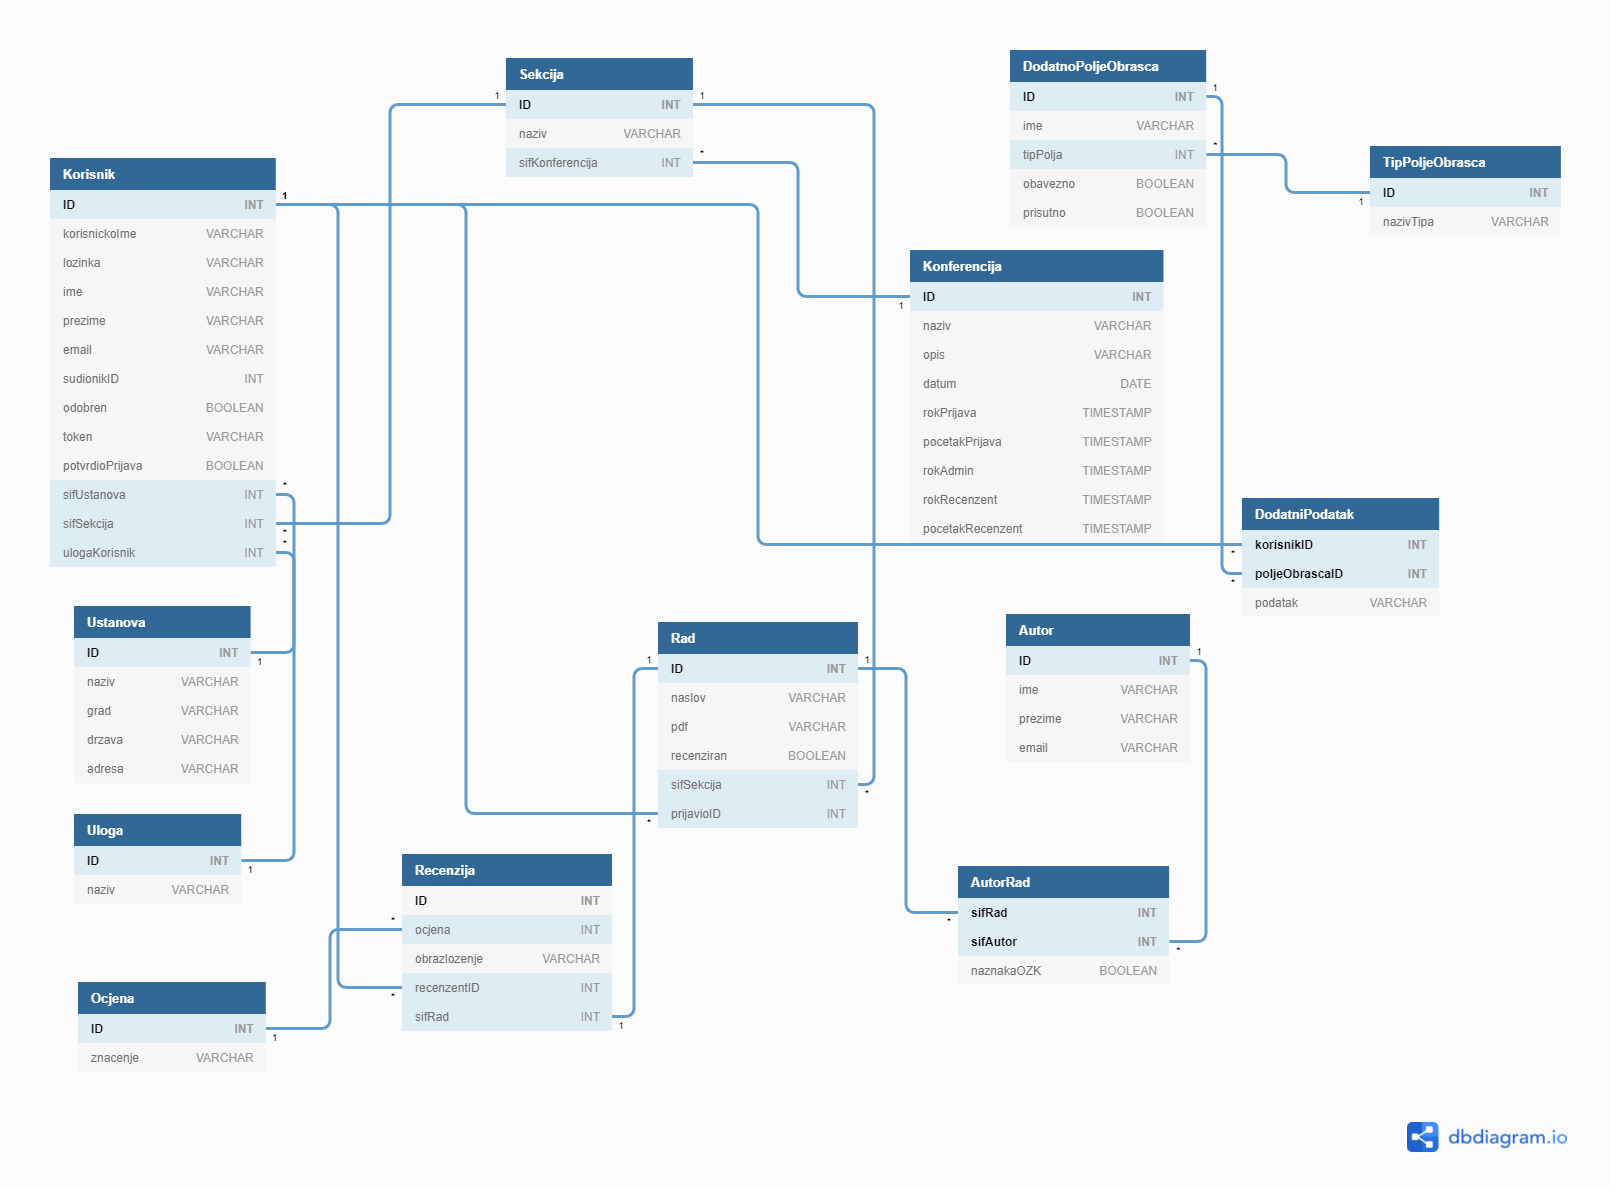
\includegraphics[width= 15 cm, keepaspectratio]{dijagrami/ZK-ER-DIJAGRAM.png} 
					\centering
					\caption{ER dijagram baze podataka}
					\label{fig:ERdijagram}
				\end{figure}
			\eject
			
			
		\section{Dijagram razreda}
		
			\textit{Potrebno je priložiti dijagram razreda s pripadajućim opisom. Zbog preglednosti je moguće dijagram razlomiti na više njih, ali moraju biti grupirani prema sličnim razinama apstrakcije i srodnim funkcionalnostima.}\\
			
			\textbf{\textit{dio 1. revizije}}\\
			
			\textit{Prilikom prve predaje projekta, potrebno je priložiti potpuno razrađen dijagram razreda vezan uz \textbf{generičku funkcionalnost} sustava. Ostale funkcionalnosti trebaju biti idejno razrađene u dijagramu sa sljedećim komponentama: nazivi razreda, nazivi metoda i vrste pristupa metodama (npr. javni, zaštićeni), nazivi atributa razreda, veze i odnosi između razreda.}\\
			
			\textbf{\textit{dio 2. revizije}}\\			
			
			\textit{Prilikom druge predaje projekta dijagram razreda i opisi moraju odgovarati stvarnom stanju implementacije}
			
			
			
			\eject
		
		\section{Dijagram stanja}
			
			
			\textbf{\textit{dio 2. revizije}}\\
			
			\textit{Potrebno je priložiti dijagram stanja i opisati ga. Dovoljan je jedan dijagram stanja koji prikazuje \textbf{značajan dio funkcionalnosti} sustava. Na primjer, stanja korisničkog sučelja i tijek korištenja neke ključne funkcionalnosti jesu značajan dio sustava, a registracija i prijava nisu. }
			
			
			\eject 
		
		\section{Dijagram aktivnosti}
			
			\textbf{\textit{dio 2. revizije}}\\
			
			 \textit{Potrebno je priložiti dijagram aktivnosti s pripadajućim opisom. Dijagram aktivnosti treba prikazivati značajan dio sustava.}
			
			\eject
		\section{Dijagram komponenti}
		
			\textbf{\textit{dio 2. revizije}}\\
		
			 \textit{Potrebno je priložiti dijagram komponenti s pripadajućim opisom. Dijagram komponenti treba prikazivati strukturu cijele aplikacije.}
	\chapter{Implementacija i korisničko sučelje}
		
		
		\section{Korištene tehnologije i alati}
		
		
			Komunikacija unutar tima odvijala se putem aplikacija \underline{WhatsApp}\footnote {\url{https://www.whatsapp.com/}} i \underline{Discord} \footnote{\url{https://discord.com}}, a s profesorom smo komunicirali putem \underline{MS Teamsa} \footnote{\url{https://www.microsoft.com/hr-hr/microsoft-teams/group-chat-software/}}.
			
			
			Za izradu UML dijagrama korišten je alat \underline{Astah Professional} \footnote {\url{https://astah.net/downloads/}} (studentska licenca), a za izradu ER dijagrama javno dostupan alat \underline{dbdiagram} \footnote {\url{https://dbdiagram.io/home}}.
			
			Verzioniranje koda olakšale su nam platforme \underline{Git} \footnote {\url{https://git-scm.com/}}  i \underline{GitLab} \footnote {\url{https://gitlab.com/}}  na kojem je dostupan udaljeni repozitorij s kojeg i na koji članovi razvojnog tima mogu preuzimati/postavljati kod i projektnu dokumentaciju.
			
			 Dokumentacija je pisana unutar okoline \underline{TeXstudio} \footnote {\url{https://www.latex-project.org/}} koja olakšava pisanje u \underline{LaTeX-u} \footnote {\url{https://www.texstudio.org/}} koji omogućuje izradu strukturiranog i preglednog dokumenta.
			
		
			Članovi tima su koristili razvojno okruženje s kojim su od ranije upoznati, \underline{Microsoft Visual Studio } \footnote {\url{https://visualstudio.microsoft.com/}}. Integrirana razvojna okruženja (\textit{engl. integrated development environment (IDE)}) programerima pružaju grafičko sučelje za pisanje koda u različitim programskih jezicima, usporedni pregled različitih projekata i druge pogodnosti poput uočljivog formatiranja koda i olakšanog otkrivanja i ispravljanja pogrešaka. 
			
			Osim ručnog testiranja aplikaciju smo testirali pomoću radnog okvira \underline{Selenium} \footnote {\url{https://www.selenium.dev/}}. Važno je biti svjestan da je nepostojanje pogreške, bez formalne verifikacije, nemoguće utvrditi.
			
			Poslužiteljska strana aplikacije implementirana je koristeći radni okvir za razvoj web aplikacija \underline{Django } \footnote {\url{https://www.djangoproject.com/}}(jezik \underline{Python 3.8} \footnote {\url{https://www.python.org/downloads/}}). Prednosti uporabe ovog (i sličnih) radnih okvira su olakšana implementacija čestih funkcionalnosti, komunikacija s bazom podataka, osigurana određena razina sigurnosti i općenito olakšana izgradnja programske potpore. Za bazu podataka odabrana je baza \underline{PostgreSQL }\footnote {\url{https://www.postgresql.org/}},  na glasu kao pouzdana i robusna relacijska baza podataka.
			Za izradu klijentske strane tradicionalno je korišten \underline{HTML}\footnote {\url{https://developer.mozilla.org/en-US/docs/Web/HTML}}, \underline{CSS}\footnote {\url{https://www.w3.org/Style/CSS/Overview.en.html}} i \underline{JavaScript} \footnote {\url{	https://www.javascript.com/}}. Izradu korisničnog sučelja olakšao nam je razvojni okvir \underline{Bootstrap}\footnote {\url{https://getbootstrap.com/}} s mnoštvom javno dostupnih stilova za često korištene HTML elemente. Pri dizajniranju izgleda stranice korištene su i SVG ikonice javno dostupne na stranici \underline{FreeSVG} \footnote {\url{https://freesvg.org/}}. 
		
			Radi pouzdanosti i neovisnosti aplikacije obavljena je virtualizacija korištenjem platforme\underline{ Docker} \footnote {\url{https://www.docker.com/}}, a objavljena je na javnom poslužitelju pomoću \underline{Digital Oceana} \footnote {\url{https://www.digitalocean.com/}}, brzorastuće platforme zasnovane na računarstvu u oblaku (\textit{engl. cloud computing}), koja između ostalih pruža uslugu objave aplikacija (\textit{engl. cloud hosting}). Na poslužitelju, tzv. \textit {dropletu}, konfigurirali smo dva kontejnera, jedan za aplikaciju i jedan za bazu podataka. \newline

		
			
			Temeljna je svrha svih navedenih tehnologija i alata ubrzati i pojednostaviti razvoj programske potpore visoke kvalitete.
					
			\eject 
		
	
		\section{Ispitivanje programskog rješenja}
			
			\textbf{\textit{dio 2. revizije}}\\
			
			 \textit{U ovom poglavlju je potrebno opisati provedbu ispitivanja implementiranih funkcionalnosti na razini komponenti i na razini cijelog sustava s prikazom odabranih ispitnih slučajeva. Studenti trebaju ispitati temeljnu funkcionalnost i rubne uvjete.}
	
			
			\subsection{Ispitivanje komponenti}
			\textit{Potrebno je provesti ispitivanje jedinica (engl. unit testing) nad razredima koji implementiraju temeljne funkcionalnosti. Razraditi \textbf{minimalno 6 ispitnih slučajeva} u kojima će se ispitati redovni slučajevi, rubni uvjeti te izazivanje pogreške (engl. exception throwing). Poželjno je stvoriti i ispitni slučaj koji koristi funkcionalnosti koje nisu implementirane. Potrebno je priložiti izvorni kôd svih ispitnih slučajeva te prikaz rezultata izvođenja ispita u razvojnom okruženju (prolaz/pad ispita). }
			
			
			
			\subsection{Ispitivanje sustava}
			
			Za testiranje sustava odabran je radni okvir Selenium IDE\footnote{\url{https://www.selenium.dev/selenium-ide/}} radi njegove jednostavnosti korištenja te sličnosti ponašanju stvarnog korisnika. Odabrani testovi usredotočeni su na administrativne zadatke sustava i pokrivaju velik broj obrazaca uporabe.\\ 
			 
			 \textbf{Ispitni slučaj 1: Dodavanje administratora}\\
			 \textbf{Ulaz:}
			 \begin{packed_item}
			 	\item {Prijava u sustav kao administrator}
			 	\item {Ulaz u administracijsko sučelje klikom na gumb u izbornoj traci}
			 	\item {Unos neispravnih korisničkih podataka novog administratora}
			 	\item {Unos ispravnih korisničkih podataka novog administratora}
			 \end{packed_item}
			 
			 \textbf{Očekivani rezultat:}
			 \begin{packed_item}
			 	\item {Uspješna prijava u sustav}
			 	\item {Otvaranje administracijskog sučelja}
			 	\item {Dojava greške o neispravnoj adresi e-pošte}
			 	\item {Potvrda o dostavi korisničkih podataka novog administratora na adresu e-pošte}
			 \end{packed_item}
			 \textbf{Rezultat: }Prijava u postojeći administratorski račun je uspješna, unos neispravne adrese e-pošte pri unosu podataka novog administratora ispravno dojavljuje grešku, a prilikom unosa ispravnih korisničkih podataka ispravno se prikazuje potvrda o dostavljenim podatcima na adresu e-pošte. Aplikacija prolazi test.\\
			
			 \textbf{Ispitni slučaj 2: Dodavanje novih sekcija}\\
			 \textbf{Ulaz:}
			 \begin{packed_item}
			 	\item {Prijava u sustav kao administrator}
			 	\item {Ulaz u administracijsko sučelje klikom na gumb u izbornoj traci}
			 	\item {Unos već postojeće sekcije}
			 	\item {Unos nove sekcije}
			 \end{packed_item}
			 \textbf{Očekivani rezultat:}
			 \begin{packed_item}
			 	\item {Uspješna prijava u sustav}
			 	\item {Otvaranje administracijskog sučelja}
			 	\item {Dojava greške o već postojećoj sekciji}
			 	\item {Nova sekcija dodanu u listu sekcija}
			 \end{packed_item}
			 \textbf{Rezultat: }Prijava u postojeći administratorski račun je uspješna i otvara se administracijsko sučelje. Pokušaj dodavanja sekcije koja već postoji ispravno javlja pogrešku o pokušaju unosa već postojeće sekcije. Unos nove sekcije je uspješan i ispravno se dodaje na listu sekcija. Aplikacija prolazi test.\\
			
			
			 \textbf{Ispitni slučaj 3: Registracija kao recenzent}\\
			 \textbf{Ulaz:}
			 \begin{packed_item}
			 	\item {Klik na gumb za registraciju u izbornoj traci}
			 	\item {Unos podataka za registraciju}
			 	\item {Odabir registracije kao recenzent}
			 \end{packed_item}
			 \textbf{Očekivani rezultat:}
			 \begin{packed_item}
			 	\item {Otvara se sučelje za registraciju}
			 	\item {Odabirom registracije kao recenzent mijenjaju se polja obrasca prijave}
			 	\item {Obavijest o potrebi da predsjedavajući potvrdi registraciju}
			 \end{packed_item}
			 \textbf{Rezultat: }Sučelje za registraciju otvara se nakon klika na gumb registracije. Nakon sto se označi gumb da se korisnik prijavljuje kao recenzent, obrazac prijave se mijenja i traži se odabir sekcije za koju se korisnik registrira. Po završetku prijave ispravno se javlja obavijest kako je potrebno da predsjedavajući potvrdi registraciju prije mogućnosti recenziranja. Aplikacija prolazi test.\\
			
			
			 \textbf{Ispitni slučaj 4: Potvrda prijave recenzenta od predsjedavajućeg\\
			 \textbf{Ulaz:}
			 \begin{packed_item}
			 	\item {Prijava u sustav kao predsjedavajući}
			 	\item {Otvaranje upravljačkog sučelja}
			 	\item {Klik na gumb "Potvrdi"}
			 \end{packed_item}
			 \textbf{Očekivani rezultat:}
			 \begin{packed_item}
			 	\item {Izborna traka se mijenja i pojavljuje se gumb za otvaranje upravljačkog sučelja predsjedavajućeg}
			 	\item {Otvara se upravljačko sučelje predsjedavajućeg}
			 	\item {Prijava se prihvaća i recenzentu šalje se e-pošta s podacima za prijavu}
			 \end{packed_item}
			 \textbf{Rezultat: }Prijavom kao predsjedavajući mijenja se izborna traka i pojavljuje se gumb za otvaranje upravljačkog sučelja predsjedavajućeg konferencije. Otvaranjem sučelja vidljiv je popis recenzenata koji čekaju potvrdu registracije. Klikom na gumb "Potvrdi" recenzentu se šalje e-pošta s potrebnim podacima za prijavu. Aplikacija prolazi test.\\
			\eject 
		
		
		\section{Dijagram razmještaja}
			
			\textbf{\textit{dio 2. revizije}}
			
			 \textit{Potrebno je umetnuti \textbf{specifikacijski} dijagram razmještaja i opisati ga. Moguće je umjesto specifikacijskog dijagrama razmještaja umetnuti dijagram razmještaja instanci, pod uvjetom da taj dijagram bolje opisuje neki važniji dio sustava.}
			 
			 
			\begin{figure}[H]
			 	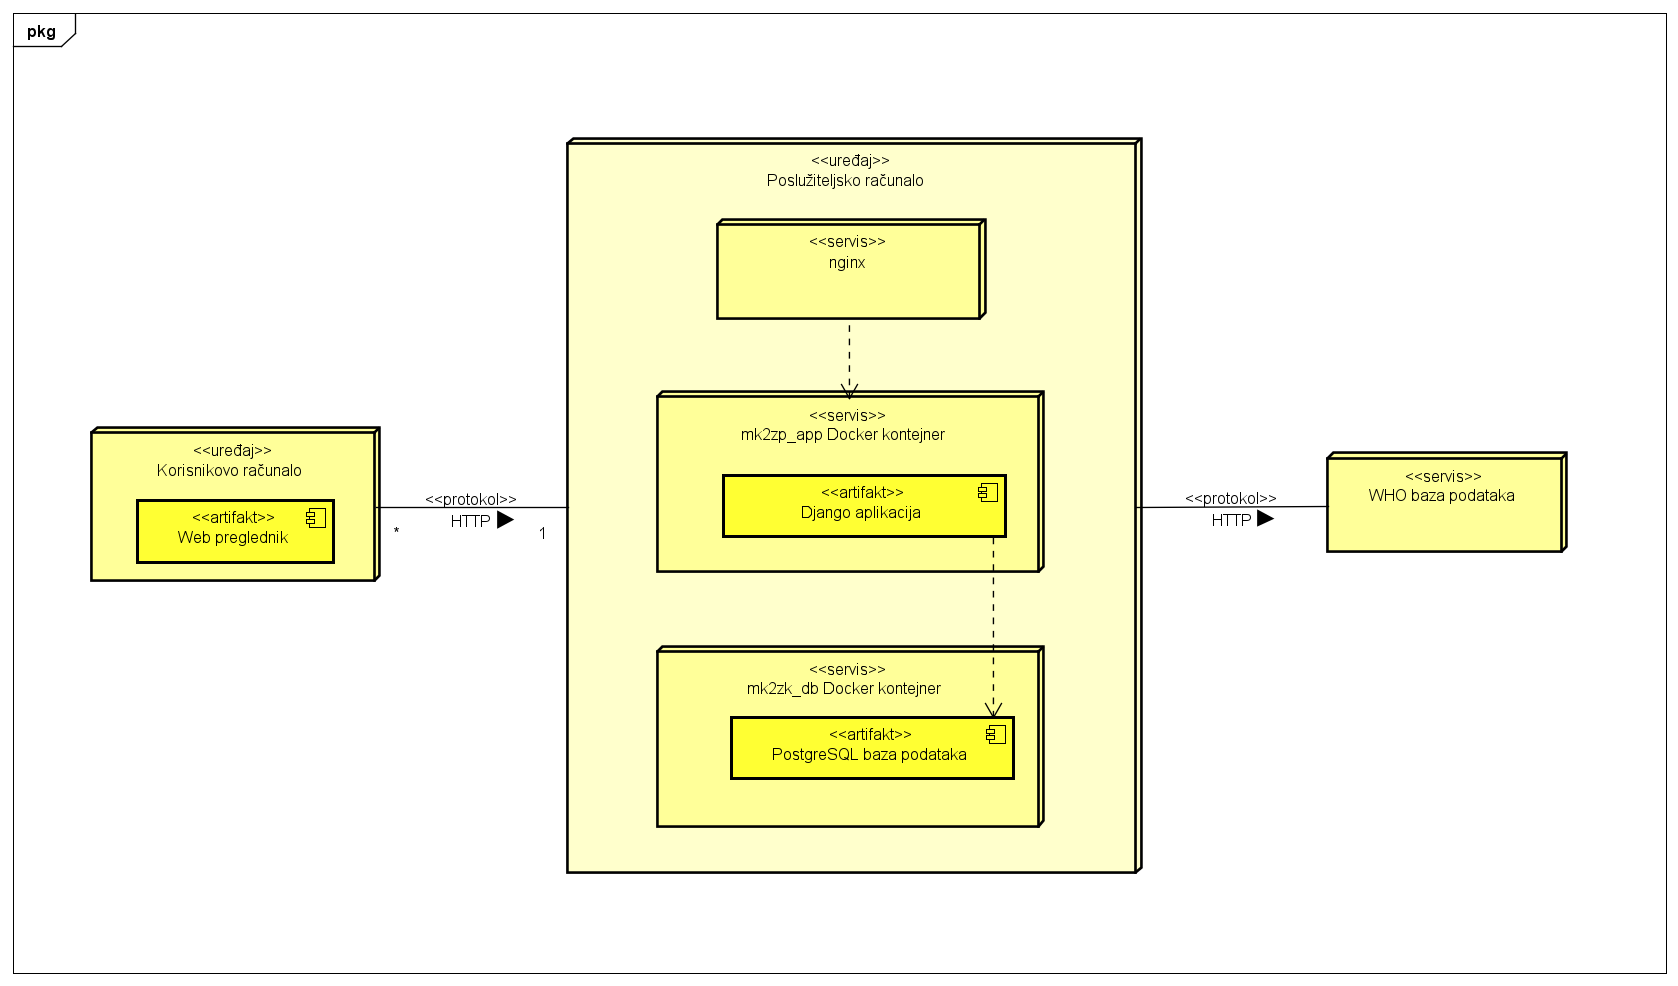
\includegraphics[width= 15 cm, height= 25 cm, keepaspectratio]{dijagrami/Diagram razmjestaja.png} 
			 	\centering
			 	\caption{Dijagram razmještaja - Znanstvena konferencija}
			 	\label{fig:act5}
			 \end{figure}
			
			\eject 
		
		\section{Upute za puštanje u pogon}
		
			\textbf{\textit{dio 2. revizije}}\\
		
			 \textit{U ovom poglavlju potrebno je dati upute za puštanje u pogon (engl. deployment) ostvarene aplikacije. Na primjer, za web aplikacije, opisati postupak kojim se od izvornog kôda dolazi do potpuno postavljene baze podataka i poslužitelja koji odgovara na upite korisnika. Za mobilnu aplikaciju, postupak kojim se aplikacija izgradi, te postavi na neku od trgovina. Za stolnu (engl. desktop) aplikaciju, postupak kojim se aplikacija instalira na računalo. Ukoliko mobilne i stolne aplikacije komuniciraju s poslužiteljem i/ili bazom podataka, opisati i postupak njihovog postavljanja. Pri izradi uputa preporučuje se \textbf{naglasiti korake instalacije uporabom natuknica} te koristiti što je više moguće \textbf{slike ekrana} (engl. screenshots) kako bi upute bile jasne i jednostavne za slijediti.}
			
			
			 \textit{Dovršenu aplikaciju potrebno je pokrenuti na javno dostupnom poslužitelju. Studentima se preporuča korištenje neke od sljedećih besplatnih usluga: \href{https://aws.amazon.com/}{Amazon AWS}, \href{https://azure.microsoft.com/en-us/}{Microsoft Azure} ili \href{https://www.heroku.com/}{Heroku}. Mobilne aplikacije trebaju biti objavljene na F-Droid, Google Play ili Amazon App trgovini.}
			
			
			\eject 
	\chapter{Zaključak i budući rad}
		
		\textbf{\textit{dio 2. revizije}}\\
		 
		 Zadatak naše grupe bio je razvoj web aplikacije za znanstvenu konferenciju koja omogućuje sudionicima konferencije prijavu znanstvenih radova, recenzentima ocjenjivanje prijavljenih radova, te predsjedavajućem konferencije pregled korisnika i odobravanje recenzenata. Nakon 15 tjedana rada u timu i razvoja aplikacije, ostvarili smo zadani cilj. Provedba projekta odvijala se u dvije faze.
		 \newline
		 \newline
		 \indent Prva faza projekta fokusirala se na izradi kvalitetne dokumentacije, što je temelj razvoja sustava i ključan element u daljnjoj implementaciji rješenja. Faza je uključivala okupljanje tima za razvoj aplikacije, dodjelu projektnog zadatka te intenzivnu izradu i razradu funkcionalnih zahtjeva te obrazaca uporabe, kao i ostale dokumentacije. Kvalitetna razrada zahtjeva aplikacije uvelike je pomogla pri daljnjem razvoju sustava. Izrađeni su potrebni dijagrami te je stvorena baza podataka specifična potrebama aplikacije, što je bio ključno pomagalo timovima zaduženim za razvoj same aplikacije. Izrada vizualnih prikaza idejnih rješenja zadatka uvelike je pomoglo razvojnim timovima pri rješavanju nedoumica u implementaciji rješenja. Razvijena je prva trećina aplikacije s registracijom, prijavom i predajom radova sudionika, što je uvelike olakšalo drugu fazu, budući da nije bilo nikakvih zaostataka.
		 \newline
		 \newline
		 \indent U drugoj fazi projekta stavljen je fokus na implementaciju rješenja za aplikaciju, temeljena na razrađenoj dokumentaciji u prethodnoj fazi. Ova je faza programerski i tehnički zahtjevnija od prve faze, te su članovi tima, zbog manjka znanja i iskustva, bili primorani samostalno učiti nove tehnologije i alate za uspješno ispunjavanje dogovorenih ciljeva. Osim realizacije rješenja, u drugoj je fazi bilo potrebno izraditi preostale dijagrame i u potpunosti uskladiti dokumentaciju s razvijenom aplikacijom kako bi budući korisnici mogli lakše koristiti sustav ili vršiti preinake nad njim. 
		 \newline
		 \newline
		 \indent Komunikacija među članovima tima odvijala se Whatsapp i Discord aplikacijama, čime smo postigli visoku informiranost svih članova grupe u svim fazama projekta, te organiziranu komunikaciju unutar pojedinih podtimova. Moguće proširenje postojećeg sustava je izrada mobilne aplikacije za konferenciju koja bi mogla, osim postojećih funkcionalnosti postojeće web aplikacije, imati dodatne mogućnosti poput povezivanja s drugim mobilnim aplikacijama. 
		 \newline
		 \newline
		 \indent Sudjelovanje na ovom projektom svim je članovima tima bilo vrijedno i kvalitetno iskustvo jer smo u kratkom i intenzivnom roku iskusili zajednički rad u timu na projektu. Također, spoznali smo važnost dobre komunikacije, koordinacije i vremenske organiziranosti, te ponajviše kvalitetne razrade problemskog zadatka. Zadovoljni smo postignutim ciljevima, iako postoji prostora za napredak i poboljšanje aplikacije, što je posljedica neiskustva članova tima na takvim projektima.
		
		\eject 
	\chapter*{Popis literature}
		\addcontentsline{toc}{chapter}{Popis literature}
	 	
 		
	
		
		\begin{enumerate}
			
			
			\item  Programsko inženjerstvo, FER ZEMRIS, \url{http://www.fer.hr/predmet/proinz}
			
			\item  I. Sommerville, "Software engineering", 8th ed, Addison Wesley, 2007.
			
			\item  T.C.Lethbridge, R.Langaniere, "Object-Oriented Software Engineering", 2nd ed. McGraw-Hill, 2005.
			
			\item  The Unified Modeling Language, \url{https://www.uml-diagrams.org/}
			
			\item  Astah Community, \url{http://astah.net/editions/uml-new}
			
			\item  Mozilla, Django introduction, \url{https://docs.djangoproject.com/en/4.0}

			\item WhatsApp (komunikacija), \url{https://www.whatsapp.com}

			\item Discord (komunikacija), \url{https://discord.com}

			\item Microsoft Teams (komunikacija), \url{https://www.microsoft.com/hr-hr/microsoft-teams}

			\item Dbdiagram, alat za izradu ER dijagrama, \url{https://dbdiagram.io/home}

			\item platforme Git i GitLab, \url{https://git-scm.com/} i \url{https://gitlab.com}

			\item LaTeX i TeXstudio, \url{https://www.latex-project.org/} i \url{https://www.texstudio.org}

			\item Visual Studio Code, \url{https://visualstudio.microsoft.co}

			\item Selenium framework, \url{https://www.selenium.dev}		
			
		\end{enumerate}

	
	
	\begingroup
	\renewcommand*\listfigurename{Indeks slika i dijagrama}
	%\renewcommand*\listtablename{Indeks tablica}
	%\let\clearpage\relax
	\listoffigures
	%\vspace{10mm}
	%\listoftables
	\endgroup
	\addcontentsline{toc}{chapter}{Indeks slika i dijagrama}


	
	\eject 
		
	\chapter*{Dodatak: Prikaz aktivnosti grupe}
		\addcontentsline{toc}{chapter}{Dodatak: Prikaz aktivnosti grupe}
		
		\section*{Dnevnik sastajanja}
		
		\textbf{\textit{Kontinuirano osvježavanje}}\\
	
		
		\begin{packed_enum}
			\item  sastanak
			
			\item[] \begin{packed_item}
				\item Datum: 11. listopada 2021.
				\item Prisustvovali: J.Gavran, L.Mujagić, M.Capan, P.D.Grujić Ostojić, R.Pintar, F.Mesić, A.Sambolek 
				\item Teme sastanka:
				\begin{packed_item}
					\item Na prvom smo se neformalnom sastanku upoznali i kratko prodiskutirali dodijeljeni projektni zadatak složivši se da nećemo predlagati vlastiti projektni zadatak.
					
					\item Okvirno smo dogovorili podjelu uloga unutar tima koju ćemo po potrebi revidirati. Članovi tima će si međusobno pomagati te će svatko imati priliku (i obvezu)
					raditi i na implementaciji i na dokumentaciji projekta. Po trenutnoj su podjeli uloga za poslužiteljsku stranu aplikacije zaduženi M.Capan i F.Mesić, za klijentsku
					stranu R.Pintar i L.Mujagić, za dokumentaciju zahtjeva A.Sambolek, za bazu podataka P.D.Grujić Ostojić te za dizajn korisničkog sučelja/korisničkog iskustva J.Gavran.
					
					\item Razgovarali smo koje bismo tehnologije i alate koristili pri razvoju aplikacije, a koje za komunikaciju unutar tima. Inicijalni je dogovor da ćemo koristiti Python,
					Bootstrap i PostgreSQL, a komunicirat ćemo preko WhatsAppa i Discorda.
				\end{packed_item}
			\end{packed_item}
			
			\item  sastanak
			\item[] \begin{packed_item}
				\item Datum: 13. listopada 2021.
				\item Prisustvovali: J.Gavran, L.Mujagić, M.Capan, P.D.Grujić Ostojić, R.Pintar, F.Mesić, A.Sambolek
				\item Teme sastanka:
				\begin{packed_item}
					\item  Na ovom inicijalnom sastanku s asistentom Miljenkom Krhenom bili su prisutni svi članovi tima i demonstrator zadužen za našu grupu, kolega Vedran Kolka.
					Asistent nam je dao osnovne informacije o načinu provedbe i kolokviranju projekta. Pozvani smo dolaziti na fakultet u terminima laboratorijskih vježbi kako bismo
					diskutirali projektno rješenje i nedoumice, a također pitanja možemo postavljati i preko platforme MS Teams.
					
				\end{packed_item}
			\end{packed_item}
			\item  sastanak
			\item[] \begin{packed_item}
				\item Datum: 25.listopada 2021.
				\item Prisustvovali: J.Gavran, L.Mujagić, M.Capan, P.D.Grujić Ostojić, R.Pintar, F.Mesić, A.Sambolek
				\item Teme sastanka:
				\begin{packed_item}
					\item Na ovom smo se online sastanku bavili izlučivanjem i analizom funkcionalnih zahtjeva. Dogovorili smo tko će raspisati funkcionalne zahtjeve, tko će napraviti tekstualni, a tko grafički prikaz (UML dijagrame) obrazaca uporabe.
					\item Raspravljali smo u o dizajnu korisničkog sučelja web-aplikacije, komentirali što nam se (ne) sviđa na nekim javno dostupnim web-stranicama za prijavu na konferencije.
				\end{packed_item}
			\end{packed_item}
		     \item  sastanak
		     \item[] \begin{packed_item}
		     		\item Datum: 3. studenoga 2021.
		     		\item Prisustvovali: J.Gavran, L.Mujagić, M.Capan, P.D.Grujić Ostojić, R.Pintar, F.Mesić, A.Sambolek
		     		\item Teme sastanka:
		     		\begin{packed_item}
		     			\item Rješavali smo neke dvojbe vezane uz konzistentnost i kompletnost funkcionalnih zahtjeva. Dogovorili smo tko će raspisati i napraviti sekvencijske dijagrame.
		     			\item Dogovorili smo početnu podjelu posla na klijentskoj i poslužiteljskoj strani aplikacije te izradi sheme baze podataka.
		     	\end{packed_item}
	    	\end{packed_item}	
    		\item  sastanak
    		\item[] \begin{packed_item}
    			\item Datum: 10. studenog 2021.
    			\item Prisustvovali: J. Gavran, L.Mujagić, R.Pintar, F.Mesić
    			\item Teme sastanka:
    			\begin{packed_item}
    				\item Definiranje i raspodjela zadataka Front-enda (Gavran, Mujagić, Pintar)
    				\item Konzultacija s Back-endom (Mesić) vezano za određene funkcionalnosti i implementaciju tih funkcionalnosti 
    			\end{packed_item}
    		\end{packed_item}	
    		\item  sastanak
    		\item[] \begin{packed_item}
    			\item Datum: 15. studenog 2021.
    			\item Prisustvovali: J. Gavran, L.Mujagić, R.Pintar, F.Mesić, P.D.Grujić Ostojić
    			\item Teme sastanka:
    			\begin{packed_item}
    				\item Diskusija o generičkim funkcionalnostima 
    				\item Dogovorene preinake u dokumentaciji i izvornom kodu
    			\end{packed_item}
    		\end{packed_item}	
    	
	    	\item  sastanak
	    	\item[] \begin{packed_item}
	    		\item Datum: 15. studenog 2021.
	    		\item Prisustvovali: J. Gavran, L.Mujagić, R.Pintar, F.Mesić, P.D.Grujić Ostojić, A.Sambolek, M.Capan
	    		\item Teme sastanka:
	    		\begin{packed_item}
	    			\item kratki timski informativni sastanak, dogovor oko finalnih izmjena generičkih funkcionalnosti prije obaveznog termina laboratorijske vježbe
	    		\end{packed_item}
	    	\end{packed_item}	
    			\item Datum: 
    			\item Prisustvovali:
    			\item Teme sastanka:
    			\begin{packed_item}
    				\item
    				\item
    			\end{packed_item}
    		\end{packed_item}	

			
			%
			
		\end{packed_enum}
		
		\eject
		\section*{Tablica aktivnosti}
		
			\textbf{\textit{Kontinuirano osvježavanje}}\\
			
			\begin{longtblr}[
					label=none,
				]{
					vlines,hlines,
					width = \textwidth,
					colspec={X[7, l]X[1, c]X[1, c]X[1, c]X[1, c]X[1, c]X[1, c]X[1, c]}, 
					vline{1} = {1}{text=\clap{}},
					hline{1} = {1}{text=\clap{}},
					rowhead = 1,
				} 
				\multicolumn{1}{c|}{} & \multicolumn{1}{c|}{\rotatebox{90}{\textbf{Marin Capan}}} & \multicolumn{1}{c|}{\rotatebox{90}{\textbf{Luka Mujagić }}} &	\multicolumn{1}{c|}{\rotatebox{90}{\textbf{Petra Dunja Grujić Ostojić }}} & \multicolumn{1}{c|}{\rotatebox{90}{\textbf{Fran Mesić}}} &	\multicolumn{1}{c|}{\rotatebox{90}{\textbf{Rea Pintar}}} & \multicolumn{1}{c|}{\rotatebox{90}{\textbf{Antonio Sambolek}}} &	\multicolumn{1}{c|}{\rotatebox{90}{\textbf{Jelena Gavran }}} \\  
				Upravljanje projektom 		& 15 & 1 & 3 & 1 & 7 & 1 & 2\\ 
				Opis projektnog zadatka 	&  & 1 & 3 &  & 1 & 1 & 3\\ 
				
				Funkcionalni zahtjevi       &  & 1 & 1 &  & 1 & 5 &  \\ 
				Opis pojedinih obrazaca 	&  & 2 & 2 &  & 6 &  & 3 \\ 
				Dijagram obrazaca 			&  &  & 6 &  &  &  &  \\ 
				Sekvencijski dijagrami 		&  &  &  &  & 6 &  &  \\ 
				Opis ostalih zahtjeva 		&  &  &  &  & 2 & 1 & 1 \\ 

				Arhitektura i dizajn sustava	 &  &  & 1 &  & 1 & 3 &  \\ 
				Baza podataka				&  &  & 7 &  &  &  &   \\ 
				Dijagram razreda 			&  &  &  &  & 3 & 4 &   \\ 
				Dijagram stanja				&  &  &  &  &  &  &  \\ 
				Dijagram aktivnosti 		&  &  &  &  &  &  &  \\ 
				Dijagram komponenti			&  &  &  &  &  &  &  \\ 
				Korištene tehnologije i alati 		& 4 &  &  & 2 &  & 2 &  \\ 
				Ispitivanje programskog rješenja 	&  &  &  &  &  &  &  \\ 
				Dijagram razmještaja			&  &  &  &  &  &  &  \\ 
				Upute za puštanje u pogon 		& 4 &  &  & 5 &  &  &  \\  
				Dnevnik sastajanja 			&  &  & 1 &  & 1 & 1 & 1 \\ 
				Zaključak i budući rad 		&  &  &  &  &  &  &  \\  
				Popis literature 			&  &  &  &  &  &  &  \\  
				&  &  &  &  &  &  &  \\ \hline 
				\textit{Dodatne stavke kako ste podijelili izradu aplikacije} 			&  &  &  &  &  &  &  \\ 
				\textit{Izrada stranica (front end)} 				&  & 25 &  &  & 12 &  & 20 \\  
				\textit{Izrada baze podataka} 		 			&  &  & 7 &  &  &  & \\  
				\textit{Spajanje s bazom podataka} 							&  &  & 5 & 5 &  &  &  \\ 
				\textit{back end} 							& 20 & 5 &  & 30 &  &  &  \\  
				 							& 43 & 35 & 36 & 43 & 40 & 18 & 30\\ 
			\end{longtblr}
					
					
		\eject
		\section*{Dijagrami pregleda promjena}
		
		\textbf{\textit{dio 2. revizije}}\\
		
		\textit{Prenijeti dijagram pregleda promjena nad datotekama projekta. Potrebno je na kraju projekta generirane grafove s gitlaba prenijeti u ovo poglavlje dokumentacije. Dijagrami za vlastiti projekt se mogu preuzeti s gitlab.com stranice, u izborniku Repository, pritiskom na stavku Contributors.}
		
	


\end{document} %naredbe i tekst nakon ove naredbe ne ulaze u izgrađen dokument 


